
\section{Cas d'utilisation : Dissémination de messages}

La diffusion de messages d'un nœud à tous les autres est une fonctionnalité
courrante des réseaux (\emph{broadcast}). La propagation épidémique
(\emph{gossip})~\cite{birman1999bimodal} constitue un moyen efficace de la
mettre en place. Sa dénomination provient de son fonctionnement : Un nœud
choisit un sous-ensemble des membres du réseau et les ``contamine'' en leur
envoyant le message; les nœuds ``infectés'' en font de même; un nœud ayant déjà
envoyé le message ne le réenvoit pas. Plus la taille du sous-ensemble choisi est
élevée, plus la probabilité selon laquelle le message parvient à tous les
membres du réseau augmente~\cite{erdos1959random}.

\begin{figure}
  \begin{center}
    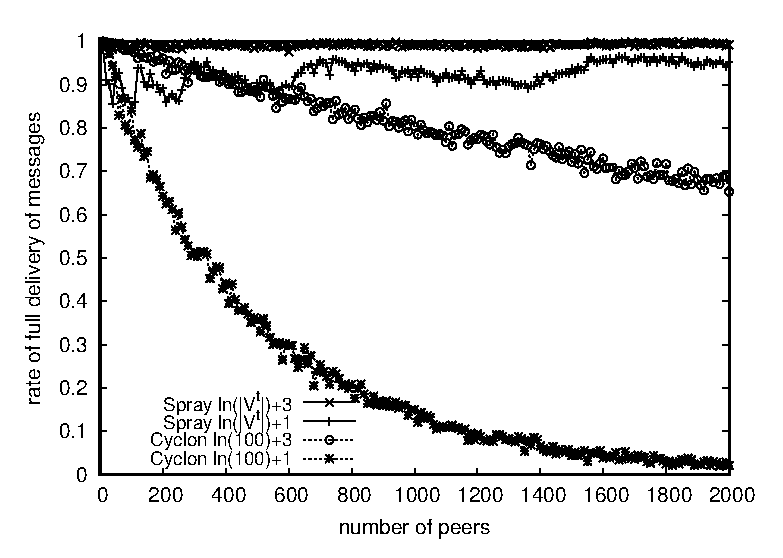
\includegraphics[width=.8\textwidth]{img/spray/hardrate.eps}
    \caption[Hard Rate]{\label{net:fig:hardrate} Hard Rate.}
  \end{center}
\end{figure}


\begin{figure}
  \begin{center}
    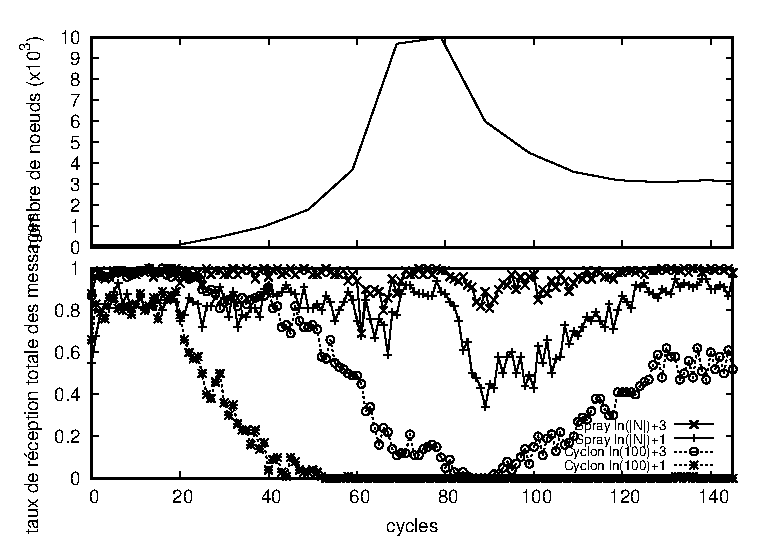
\includegraphics[width=.8\textwidth]{img/spray/peak.eps}
    \caption[Peak]{\label{net:fig:peak} Peak.}
  \end{center}
\end{figure}


%%% Local Variables:
%%% mode: latex
%%% TeX-master: "../../paper"
%%% End:
